\chapter{Regulacja procesu}
	\label{ch:reg}
	
	\section{Implementacja NPL}
		\label{sec:NPL}
		NPL jest algorytmem regulacji predykcyjnym z Nieliniową predykcją i z linearyzacją oznacza to że do wyznaczania trajektori swobodnej (która zależy tylko od przeszłych sterowań) używamy nieliniowego modelu neuronowego:
		\begin{equation}
		\begin{tabular}{l}
		$y^0(k+1)=w20+w2*tanh(w10+w1*x(k))+dk$
		\end{tabular}
		\label{eq:NPL_y0}
		\end{equation}
		gdzie
		\begin{equation}
		\begin{tabular}{l}
		$dk = y(k)-y^M(k)$
		\end{tabular}
		\label{eq:dk}
		\end{equation}
		\begin{equation}
		\begin{tabular}{l}
		$x(k)=$ $\begin{bmatrix}u(min(k-\tau+n,k-1))\\u(min(k-\tau-1+n,k-1\\y(k-1+n)\\y(k-2+n)))\end{bmatrix}$
		\end{tabular}
		\label{eq:wesn}
		\end{equation}
		$n=$ ilość chwil w przyszłóść.
		Warto dodać, że we wzore \ref{eq:wesn} dla chwil czasu dalszych od $k$ zakłada się że $y(p>k)=y^0(p)$.\\
		Aby móc rozwiązać algorytm analitycznie dokonuje się linearyzacji predykcji wyjścia modelu w przyszłości. Współczynniki $b_3$,$b_4$,$a_1$,$a_2$ we wzorze
		\begin{equation}
		\begin{tabular}{l}
		$y(k)=b_3u(k-\tau=k-3)+b_4(k-\tau-1=k-4)-a_1y(k-1)-a_2y(k-2)$
		\end{tabular}
		\label{eq:NPL_wyjscielinear}
		\end{equation}
		
		
	\section{Strojenie NPL}
		\label{sec:stroj_NPL}
		
		\begin{figure}[h!]
			\centering
			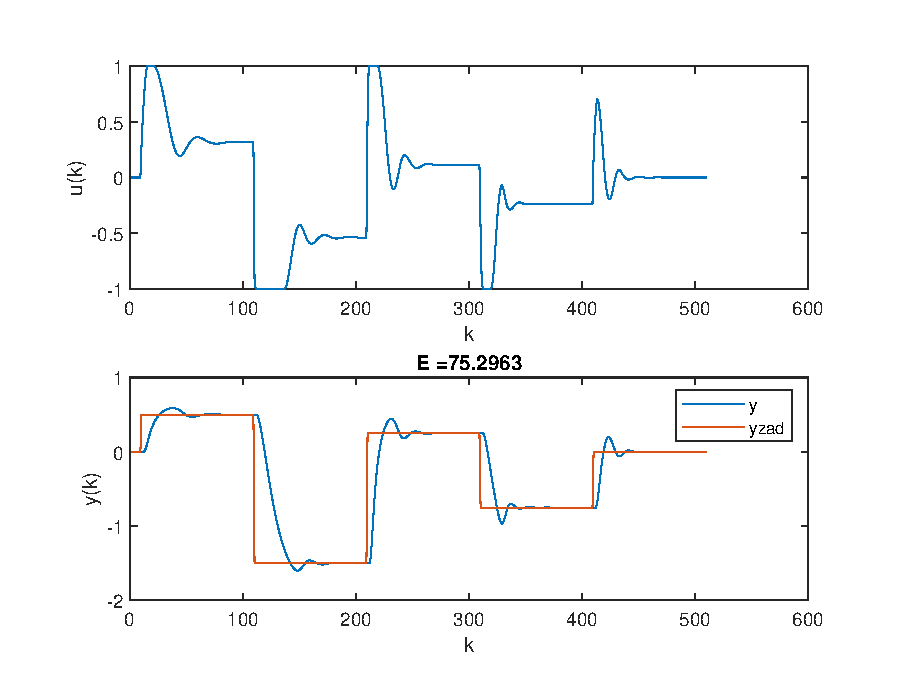
\includegraphics[width=\linewidth]{img/strojenieNPL_N_10_Nu_2_lam_1.eps}
			\caption{Działanie regulatora NPL z nastawami N=10, Nu=2, $\lambda$=1}
			\label{fig:NPL0}
		\end{figure}
		
		\begin{figure}[h!]
			\centering
			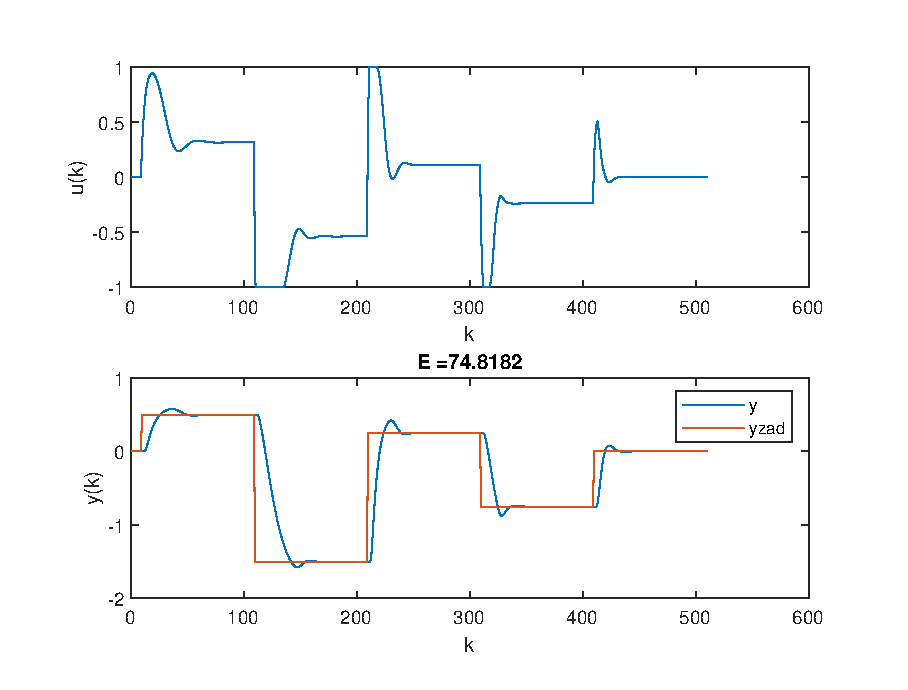
\includegraphics[width=\linewidth]{img/NPLN20.eps}
			\caption{Działanie regulatora NPL z nastawami N=20, Nu=2, $\lambda$=1}
			\label{fig:NPL1}
		\end{figure}
		
		\begin{figure}[h!]
			\centering
			\includegraphics[width=\linewidth]{img/NPLNu1.eps}
			\caption{Działanie regulatora NPL z nastawami N=20, Nu=1, $\lambda$=1}
			\label{fig:NPL2}
		\end{figure}
		
		\begin{figure}[h!]
			\centering
			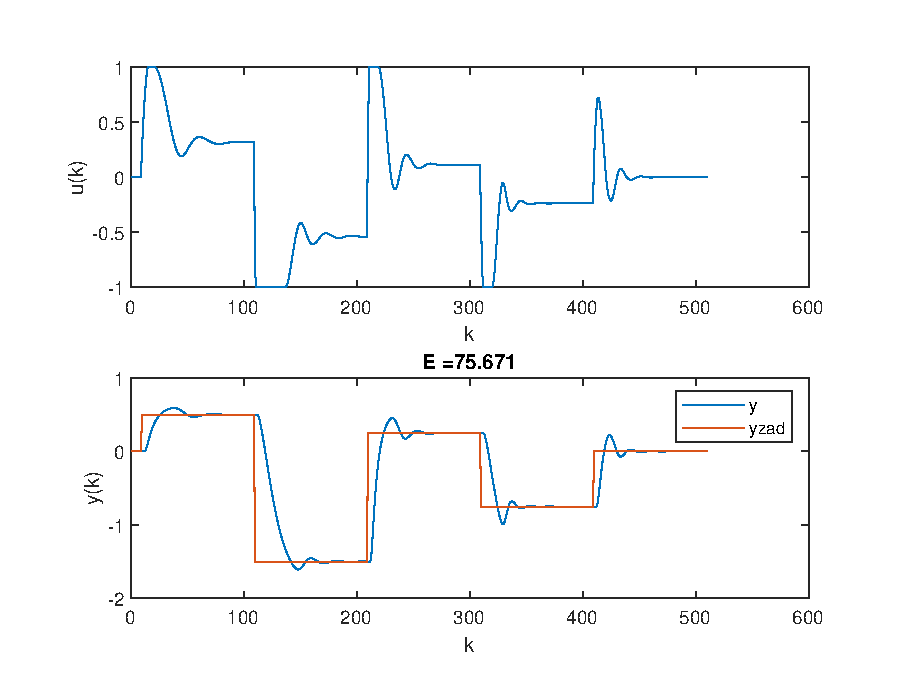
\includegraphics[width=\linewidth]{img/NPLNu3.eps}
			\caption{Działanie regulatora NPL z nastawami N=20, Nu=3, $\lambda$=1}
			\label{fig:NPL3}
		\end{figure}
		
		\begin{figure}[h!]
			\centering
			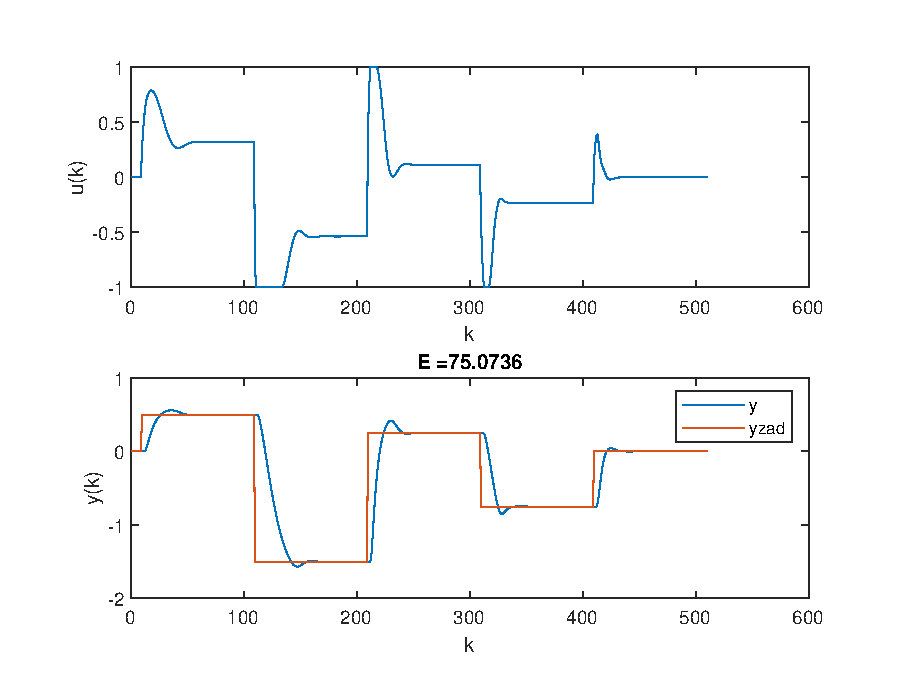
\includegraphics[width=\linewidth]{img/NPLlam2.eps}
			\caption{Działanie regulatora NPL z nastawami N=20, Nu=2, $\lambda$=2}
			\label{fig:NPL4}
		\end{figure}
		
		
	\section{GPC}
		\label{sec:GPC}
		
		\begin{figure}[h!]
			\centering
			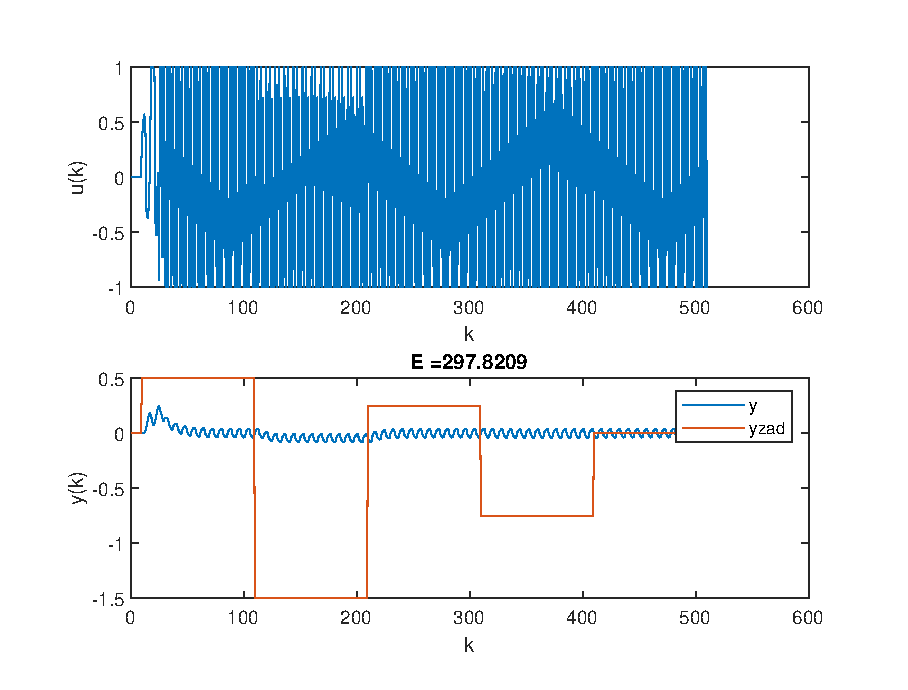
\includegraphics[width=\linewidth]{img/GPC.eps}
			\caption{Działanie regulatora GPC z nastawami N=20, Nu=2, $\lambda$=2}
			\label{fig:GPC}
		\end{figure}
		
		\begin{figure}[h!]
			\centering
			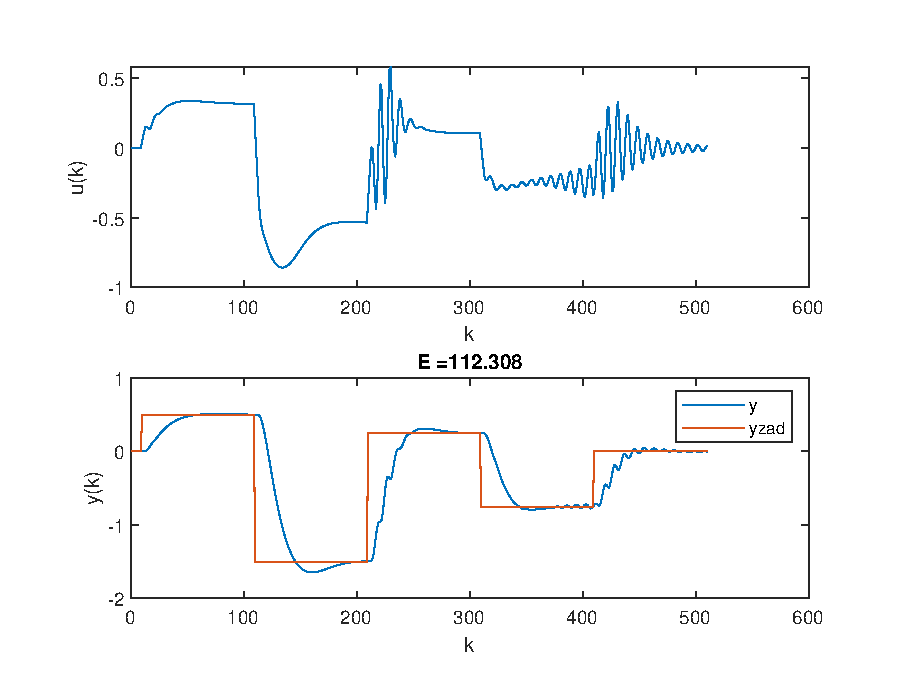
\includegraphics[width=\linewidth]{img/GPC100.eps}
			\caption{Działanie regulatora GPC z nastawami N=20, Nu=2, $\lambda$=100}
			\label{fig:GPC100}
		\end{figure}